% mainfile: ../../main.tex
\chapter{Monte Carlo and \texorpdfstring{\acrshort{gksl}}{GKSL} master equation simulations}\label{ch:app:ff:time_domain_methods}
\AutoLettrine{In} this appendix, we lay out two common time-domain simulation methods of noisy quantum dynamics for completeness; direct simulation of the \gls{gksl} master equation and stochastic \gls{mc} simulation of the Schrödinger equation.

\section{Simulation methods}\label{sec:app:ff:time_domain_methods}
\subsection{\texorpdfstring{\acrshort{gksl}}{GKSL} master equation}\label{subsec:app:ff:time_domain_methods:gksl}
To validate the fidelity for white noise, we use a \gls{gksl} master equation~\cite{Lindblad1976,Gorini1976} in superoperator form.
We represent linear maps $\mc{A}: \rho\rightarrow\mc{A}(\rho)$ by matrices in the Liouville representation following \cref{eq:ff:liouville_representation}
and operators as column vectors (\ie, generalized Bloch vectors) as
\begin{equation}\label{eq:app:ff:bloch_vector}
    \rho_i \coloneqq \tr(\sigma_i\rho),
\end{equation}
allowing us to write the Lindblad equation
\begin{equation}\label{eq:app:ff:lindblad:hilbert}
    \dv{t}\rho(t) = -\i\comm{H(t)}{\rho(t)} + \sum_\alpha \gamma_\alpha\left(L_\alpha\rho(t) L_\alpha\adjoint - \frac{1}{2}\acomm{L_\alpha\adjoint L_\alpha}{\rho(t)}\right)
\end{equation}
as a linear differential equation in matrix form,
\begin{equation}\label{eq:app:ff:lindlbad:liouville}
    \dv{t}\rho_i(t) = \sum_j\left(-\i\mc{H}_{ij}(t)+ \sum_\alpha \gamma_\alpha \mc{D}_{\alpha, ij}\right)\rho_j(t).
\end{equation}
Here, $\mc{H}_{ij}(t) = \tr(\sigma_i\comm{H(t)}{\sigma_j})$ and $\mc{D}_{\alpha, ij} = \tr\left(\sigma_i L_\alpha\sigma_j L_\alpha\adjoint - \frac{1}{2}\sigma_i \acomm{L_\alpha\adjoint L_\alpha}{\sigma_j}\right)$.
The $\gamma_\alpha$ are coupling constants to the noise bath and can be related to the amplitude of the \gls{psd}.
For Hermitian $L_\alpha$, the solution to \cref{eq:app:ff:lindblad:hilbert} is a \gls{cptp} as well as unital map.
\Cref{eq:app:ff:lindlbad:liouville} is readily solved under the approximation of piecewise constant timesteps $\Delta t_g = t_{g} - t_{g-1}$ and one obtains for the complete superpropagator
\begin{equation}\label{eq:app:ff:lindblad:propagator}
    \liouvU(t_{g}, t_{g-1}) = \exp\left\{ \left(-\i\mc{H}(t_g) + \sum_\alpha\gamma_\alpha\mc{D}_\alpha\right) \Delta t_g \right\}
\end{equation}
with
\begin{equation}
    \liouvU(\tau) = \prod_{g=G}^1\liouvU(t_{g}, t_{g-1}).
\end{equation}
The entanglement fidelity can then be computed as $\entfid = d^{-2}\tr(\liouvQ\adjoint\liouvU)$, where \liouvQ is the superpropagator due to the Hamiltonian evolution alone (\ie, the ideal evolution without noise), and \avgfid obtained using \cref{eq:ff:fidelity:avg-ent}.

\subsection{\texorpdfstring{\acrshort{mc}}{MC} Schrödinger equation}\label{subsec:app:ff:time_domain_methods:mc}
In a \gls{mc} simulation, we work with single realizations of the noise Hamiltonian in \cref{eq:ff:hamiltonian:noise} and solve the Schrödinger equation governed by it.
This results in unitary dynamics.
The ensemble-averaged dynamics are then obtained by randomly drawing many realizations, solving the Schrödinger equation and computing the desired quantities for each, before finally averaging over all realizations.
To sample the \gls{psd} faithfully, the piecewise constant time step needs to be significantly smaller than in a noise-free simulation in order to resolve high frequencies of the noise (\cf \cref{ch:speck:theory}).
In practice, we generate time traces of the noise fields by drawing pseudo-random numbers from a distribution whose \gls{psd} is $S(f)$.
To do this, we draw complex, normally distributed samples in frequency space (\ie white noise), scale it with the \gls{asd}, and finally perform the inverse Fourier transform.
We then solve the Schrödinger equation by diagonalizing the full Hamiltonian $H(t) = \Hc(t) + \Hn(t)$ and computing the propagator for one noise realization as
\begin{equation}\label{eq:app:ff:mc:propagator}
    U(t) = \prod_g V\gth{g}\exp\left(-\i\Omega\gth{g}\Delta t_\mr{MC}\right) V^{(g)\dagger},
\end{equation}
where $V\gth{g}$ is the unitary matrix of eigenvectors of $H(t)$ during time segment $g$ and $\Omega\gth{g}$ the diagonal matrix of eigenvalues.
We can then obtain an estimate for the entanglement fidelity \entfid as
\begin{equation}
    \ev{\entfid} = \ev{\abs{\tr(Q\adjoint U(\tau))}^2},
\end{equation}
and \avgfid again from \cref{eq:ff:fidelity:avg-ent}.
Here, $Q\equiv\Uc(t=\tau)$ is the noise-free propagator at time $\tau$ of completion of the circuit and $\ev{\placeholder}$ denotes the ensemble average over $N$ Monte Carlo realizations of \cref{eq:app:ff:mc:propagator}, \ie, $\ev{A}=N\inverse\sum_{i=1}^N A_i$.
The standard error of the mean can be obtained as $\sigma_{\ev{\avgfid}} = \sigma_{\avgfid} / \sqrt{N}$ with $\sigma_{\avgfid}$ the standard deviation over the Monte Carlo traces.

\section{Validation of \texorpdfstring{\acrshort{qft}}{QFT} fidelities}\label{sec:app:ff:time_domain_methods:qft_validation}
In this section, we perform \gls{gksl} master equation and \gls{mc} simulations to verify the fidelities predicted for the \gls{qft} circuit in \cref{sec:ff:examples:qft}.
We focus on noise exclusively on the third qubit, entering through the noise operator $B_\alpha\equiv\sigma_y\gth{3}$.

We assemble the \gls{qft} circuit discussed in the main text from a minimal gate set consisting of three atomic gates, $\mathbb{G} = \lbrace\mr{X}_{i}(\flatfrac{\pi}{2}),\mr{Y}_{i}(\flatfrac{\pi}{2}),\mr{CR}_{ij}(\flatfrac{\pi}{2^3})\rbrace$ on or between qubits $i$ and $j$.
We consider a simple model involving four single-spin qubits with in-phase (I) and quadrature (Q) single-qubit control and nearest neighbor exchange coupling so that the control Hamiltonian reads
\begin{equation}\label{eq:app:ff:control_hamiltonian:qft}
    \Hc(t) = \sum_{\langle i,j\rangle} I_i(t)\sx\gth{i} + Q_i(t)\sy\gth{i} + J_{ij}(t)\sz\gth{i}\otimes\sz\gth{j}
\end{equation}
where $\sigma_\alpha\gth{i}$ is the trivial extension of the Pauli matrix $\sigma_\alpha$ of qubit $i$ to the full tensor product Hilbert space.
For simplicity, we assume periodic boundary conditions so that qubits 1 and 4 are nearest neighbors as well.
Similarly, we define the noise Hamiltonian as
\begin{equation}\label{eq:app:ff:noise_hamiltonian:qft}
    \Hn(t) = \sum_{\langle i,j\rangle} b_{I}(t)\sx\gth{i} + b_{Q}(t)\sy\gth{i} + b_{J}(t)\sz\gth{i}\otimes\sz\gth{j}
\end{equation}
with the noise fields $b_{\alpha}(t)$ for $\alpha\in\{I,Q,J\}$.

For the \gls{gksl} master equation, we set $L_\alpha\equiv\sigma_y\gth{3}$ as well as $\gamma_\alpha\equiv\flatfrac{S_0}{2}$ with $S_0$ the amplitude of the one-sided noise \gls{psd} so that $S(\omega) = S_0$.
For the \gls{mc} simulation, we explicitly generate time traces of $b_Q(t)$ (\cf \cref{eq:app:ff:noise_hamiltonian:qft}).
We choose an oversampling factor of 16 so that the time discretization of the simulation is $\Delta t_\mr{MC} = \flatfrac{\Delta t}{16} = \qty{62.5}{\pico\second}$ ($\Delta t = \qty{1}{\nano\second}$ is the time step of the pulses used in the \gls{ff} simulation), leading to a highest resolvable frequency of $\fmax = \qty{16}{\giga\hertz}$.
Conversely, we increase the frequency resolution by sampling a time trace longer by a given factor, giving frequencies below \fmin (\qty{16}{\kilo\hertz} for pink, \qty{0}{\hertz} for white noise) weight zero, and truncating it to the number of time steps in the algorithm times the oversampling factor.
This yields a time trace with frequencies $f\in [\fmin, \fmax]$ and a given resolution (we choose $\df = \qty{160}{\hertz}$).
For reference, we show the fidelity filter functions for the circuit with and without echo pulses in this frequency band in \cref{fig:app:qft_ff}.

\begin{figure}
    \centering
    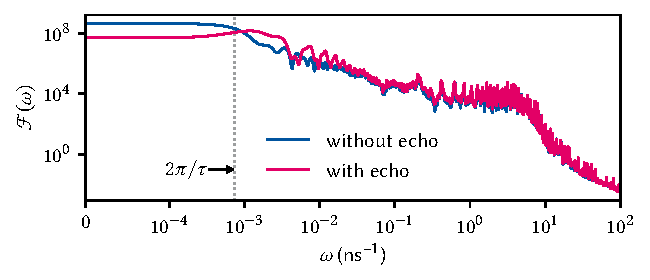
\includegraphics{img/pdf/filter_functions/qft_filter_function_Y3}
    \caption[\imgsource{img/py/filter_functions/quantum_fourier_transform.py}]{
        Filter functions for noise operator $\sigma_y\gth{3}$ for the \gls{qft} circuit without (blue) and with (magenta) additional echo pulses.
        Introducing the echoes shifts spectral weight towards higher frequencies, reducing the DC level of the filter function by two orders of magnitude and thus leading to an improved fidelity for \oneoverf noise.
    }
    \label{fig:app:qft_ff}
\end{figure}
\begin{table*}
    \centering
    \renewcommand\arraystretch{1.25}
    \caption{
        Infidelities $\avginfid = 1-\avgfid$ of the \gls{qft} circuit due to noise on $\sigma_y\gth{3}$.
        \Gls{mc} values are averages over $N=1000$ random traces and have a relative error of \qty{3}{\percent}.
        We included frequencies in the range of $\omega\in [0, 100]\,\unit{\per\nano\second}$ for white noise, and $\omega\in [\qty{100}{\per\milli\second}, \qty{100}{\per\nano\second}]$ for pink noise.
        \Gls{ff} values are computed with $n_\omega=1000$ samples logarithmically distributed over the same interval.
        Prefactors in the power law $S(\omega)= A\omega^\alpha$ are \qty{2e-6}{\per\nano\second} and \qty{1e-9}{\per\nano\second\squared}, respectively.
    }
    \label{tab:app:fidelities}
    % This table is automatically generated by img/py/filter_functions/qft_monte_carlo.py 
 \begin{tabular}{l *{4}{S[table-format=1.2e+1,round-mode=figures,round-precision=3]}}
\toprule
 & \multicolumn{2}{c}{\textsc{White noise}} & \multicolumn{2}{c}{\oneoverf \textsc{noise}} \\
\cmidrule(lr){2-3}\cmidrule(lr){4-5}
\textsc{Method} & \textsc{Without echo} & \textsc{With echo} & \textsc{Without echo} & \textsc{With echo} \\
\midrule
\acrshort{gksl} & 8.380261e-03 & 8.380835e-03 & {---} & {---} \\
\acrshort{mc} & 8.727031e-03 & 7.986534e-03 & 2.093929e-02 & 4.272077e-03 \\
\acrshort{ff} & 8.377560e-03 & 8.403532e-03 & 2.115425e-02 & 4.459941e-03 \\
\bottomrule
\end{tabular}

\end{table*}

\Cref{tab:app:fidelities} compares the infidelities $\infid=1-\fid$ from \gls{gksl} and \gls{mc} simulations to the filter function predictions following \cref{eq:ff:infidelity:ent}.
Note that the precise value of the filter function result depends quite sensitively on the frequency sampling due to the sharp peaks in the gigahertz range (\cref{fig:app:qft_ff}).
As the table shows, both the \gls{gksl} and the \gls{mc} calculations agree well with the predictions made by our filter-function formalism.
